\documentclass[11pt,a4paper]{article}
\usepackage[utf8]{inputenc}
\usepackage[margin=1in]{geometry}
\usepackage{authblk}
\usepackage{amsmath}
\usepackage{graphicx}
\usepackage{hyperref}
\usepackage{booktabs}
\usepackage{microtype}
\usepackage[backend=biber,style=ieee]{biblatex}
\addbibresource{aroma.bib}

\title{\textbf{AROMA: An Affective Role Ontology for Mental Health Agents}}
\author[1]{Zac [Author]}
\affil[1]{University [Affiliation]}
\date{March 2026}

\begin{document}

\maketitle

\begin{abstract}
Recent years have seen a proliferation of conversational AI systems designed for mental health support. However, these systems often suffer from ``role-locking''---assuming a static identity that fails to meet users' dynamic relational needs. We present \textbf{AROMA (Affective Role Ontology for Mental health Agents)}, a three-dimensional taxonomy that separates \textit{what} is given (Support Type) from \textit{who} the AI is being (Care Role). Our findings reveal a structural \textbf{Authority-Agency Paradox}: a failure mode where systems claim clinical authority but lack the agency to fulfill the role’s obligations. We demonstrate the necessity of AROMA through literature synthesis and computational validation on the 18,376-turn ESConv corpus.
\end{abstract}

\section{Introduction}
Conversational AI for mental health is at a crossroads. While agents like Woebot provide evidence-based interventions, they typically operate under a single, static system-level identity. 

Following Blumer \cite{blumer1969symbolic} and Mead \cite{mead1934mind}, we argue that care is enacted through \textit{role-taking}---the process by which an actor reads the user's expressed state and calibrates their stance accordingly. Current AI role-rigidity stems from a conceptual conflation of Support Type \cite{cutrona1992social} and Care Role \cite{biddle1986recent}. This conflation obscures the \textbf{Authority-Agency Paradox}: users project clinical authority onto an agent, but the agent lacks the structural agency \cite{parsons1951social} to fulfill that role's social obligations.

\section{The AROMA Taxonomy}
AROMA defines three orthogonal dimensions of AI-mediated care:

\subsection{D1: Support Type}
The content of support, derived from Cutrona and Suhr \cite{cutrona1992social} and Lazarus and Folkman \cite{lazarus1984stress}.

\subsection{D2: Care Role}
The relational stance adopted by the agent, grounded in symbolic interactionism \cite{blumer1969symbolic}. We identify six stable care roles (Table \ref{tab:roles}).

\begin{table}[h!]
    \centering
    \small
    \begin{tabular}{lp{4cm}p{4cm}l}
    \toprule
    \textbf{Role} & \textbf{Description} & \textbf{Identification Markers} & \textbf{Paradox Risk} \\
    \midrule
    Listener & Receptive, non-directive & Minimal encouragers, follows user lead. & Low \\
    Reflective Partner & Socratic, exploratory & Cognitive reappraisal, mirroring patterns. & Low \\
    Coach & Directive, motivating & Goal-setting, change-talk (MI). & Moderate \\
    Advisor & Authoritative, expertise-led & Psychoeducation, direct advice. & \textbf{High} \\
    Companion & Warm, persistent presence & Reciprocal disclosure, shared longitudinal references. & Low \\
    Navigator & Practical guide & Resource listing, triage questions. & \textbf{High} \\
    \bottomrule
    \end{tabular}
    \caption{The six AROMA Care Roles (D2).}
    \label{tab:roles}
\end{table}

\subsection{D3: Support Strategy}
The turn-by-turn conversational tactics \cite{hill2009helping, liu2021towards}.

\section{Methodology}
We performed a structured literature synthesis \cite{nickerson2013taxonomy} of 203 research papers. These roles are operationalized through a multitask neural classifier on the ESConv corpus \cite{liu2021towards}.

\section{Empirical Results}
Our computational results validate that Care Roles are sequence-level properties.

\begin{figure}[h!]
    \centering
    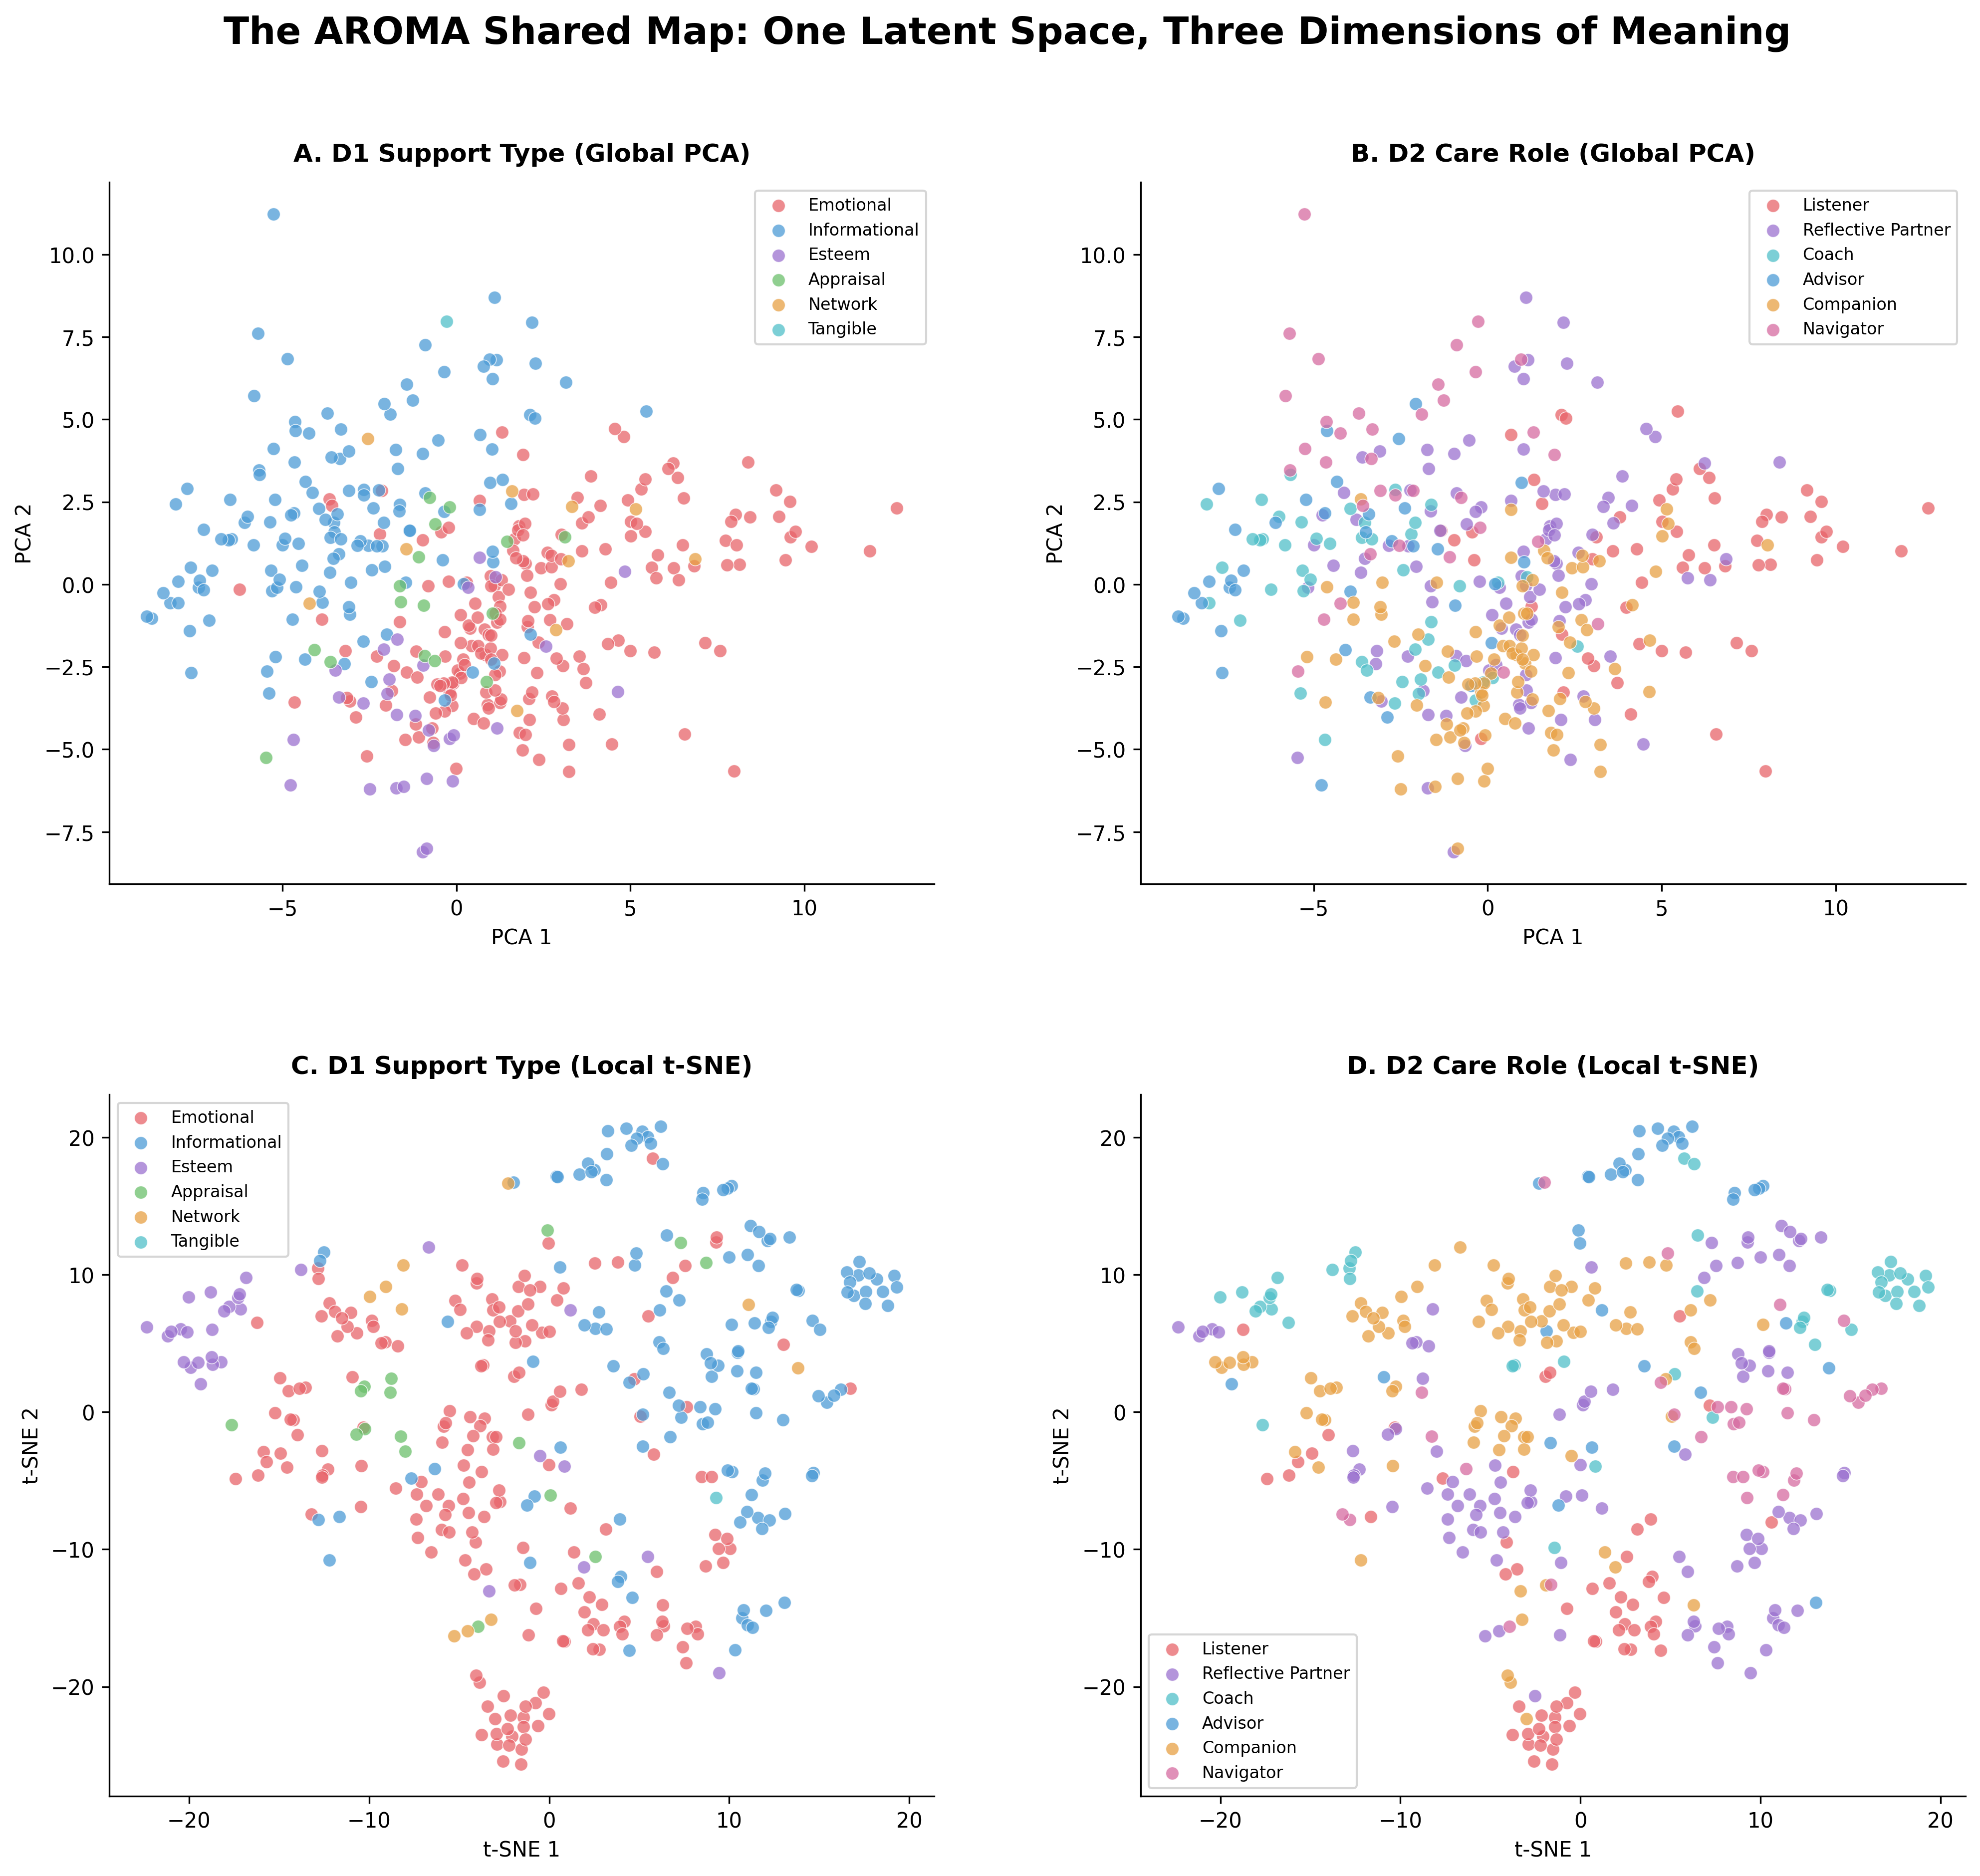
\includegraphics[width=0.8\textwidth]{../../phase_5_computational_operationalization/figures/final/combined_shared_map.png}
    \caption{The AROMA Shared Map: Unified latent space organization (N=18,376).}
\end{figure}

\begin{figure}[h!]
    \centering
    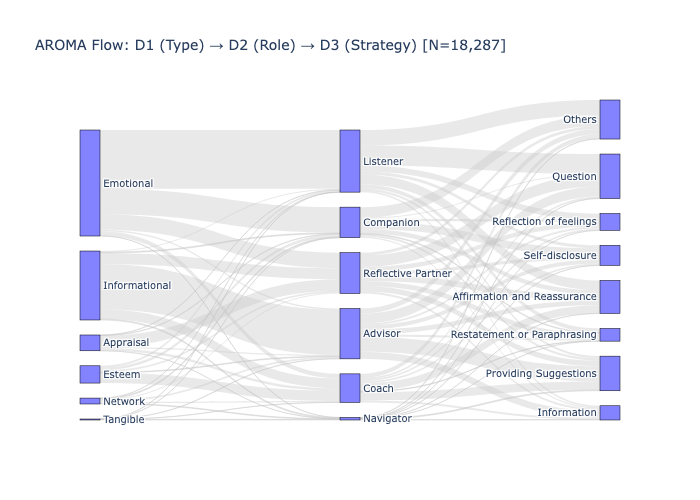
\includegraphics[width=0.8\textwidth]{../../phase_5_computational_operationalization/figures/final/full_sankey.png}
    \caption{Global AROMA Flow: Multidimensional operationalization flow.}
\end{figure}

\section{Conclusion}
AROMA provides a roadmap for designing flexible, role-aware mental health agents that can navigate the Authority-Agency Paradox safely while matching the dynamic needs of users in distress.

\printbibliography

\end{document}
